In order to test our program against human players, we will develop an application implementing a graphical user interface (\emph{GUI} or also \emph{UI}).
Figure \ref{fig:UCD_Play} represents the interactions between the player and the UI.
It will interface directly with the model, and will be controllable by the human with the mouse or keyboard, in a manner as intuitive as possible.
Thanks to this UI, the user will be able to choose between a one-player mode, a two-plaer mode and a demonstration mode.
This last mode consists in a match between two AIs, and will be helpful to compare different AIs.
The user will also be able to choose and configure the AIs, if we have time to develop more than one.

\begin{figure}[!h]
\centering
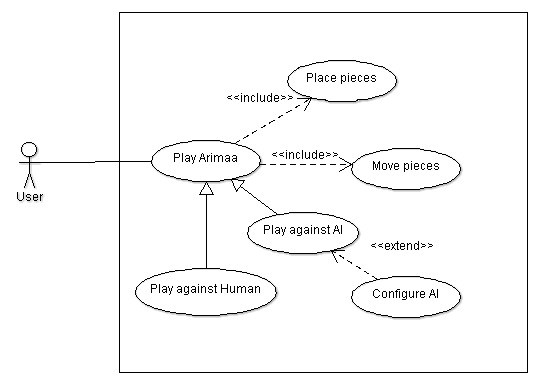
\includegraphics[width=\textwidth]{2General_Architecture/2.1Behaviour_of_the_Game/Pictures/Application_UCD}
\caption{The user-case diagram describing the interactions made possible by the UI}
\label{fig:UCD_Play}
\end{figure}